%
% Template Laporan Skripsi/Thesis 
%
% @author  Andreas Febrian, Lia Sadita 
% @version 1.03
%
% Dokumen ini dibuat berdasarkan standar IEEE dalam membuat class untuk 
% LaTeX dan konfigurasi LaTeX yang digunakan Fahrurrozi Rahman ketika 
% membuat laporan skripsi. Konfigurasi yang lama telah disesuaikan dengan 
% aturan penulisan thesis yang dikeluarkan UI pada tahun 2008.
%

%
% Tipe dokumen adalah report dengan satu kolom. 
%
\documentclass[12pt, a4paper, onecolumn, oneside, final]{report}

% Load konfigurasi LaTeX untuk tipe laporan thesis
\usepackage{style/uithesis}
\usepackage{natbib}
\usepackage{import}
% Load konfigurasi khusus untuk laporan yang sedang dibuat
%-----------------------------------------------------------------------------%
% Informasi Mengenai Dokumen
%-----------------------------------------------------------------------------%
% 
% Judul laporan. 
\var{\judul}{Strategi Penerapan Pola Model-View-Controller Pada Pengembangan Software Product Line
             Berbasis Web Dengan Menggunakan Abstract Behavioural Spesification}
% 
% Tulis kembali judul laporan, kali ini akan diubah menjadi huruf kapital
\Var{\Judul}{Strategi Penerapan Pola Model-View-Controller Pada Pengembangan Software Product Line
             Berbasis Web Dengan Menggunakan Abstract Behavioural Spesification}
% 
% Tulis kembali judul laporan namun dengan bahasa Ingris
\var{\judulInggris}{Integrating Model-View-Controller design pattern and Delta Modelling
                    for Web-Based Software Product Line Engineering}

% 
% Tipe laporan, dapat berisi Skripsi, Tugas Akhir, Thesis, atau Disertasi
\var{\type}{Proposal Thesis}
% 
% Tulis kembali tipe laporan, kali ini akan diubah menjadi huruf kapital
\Var{\Type}{Proposal Thesis}
% 
% Tulis nama penulis 
\var{\penulis}{Salman El Farisi}
% 
% Tulis kembali nama penulis, kali ini akan diubah menjadi huruf kapital
\Var{\Penulis}{Salman El Farisi}
% 
% Tulis NPM penulis
\var{\npm}{1306346720}
% 
% Tuliskan Fakultas dimana penulis berada
\Var{\Fakultas}{Ilmu Komputer}
\var{\fakultas}{Ilmu Komputer}
% 
% Tuliskan Program Studi yang diambil penulis
\Var{\Program}{Magister Ilmu Komputer}
\var{\program}{Magister Ilmu Komputer}
\var{\programEng}{Master of Computer Science}
% 
% Tuliskan tahun publikasi laporan
\Var{\bulanTahun}{Juni 2014}
% 
% Tuliskan gelar yang akan diperoleh dengan menyerahkan laporan ini
\var{\gelar}{Magister Ilmu Komputer}
% 
% Tuliskan tanggal pengesahan laporan, waktu dimana laporan diserahkan ke 
% penguji/sekretariat
\var{\tanggalPengesahan}{21 Juni 2013} 
% 
% Tuliskan tanggal keputusan sidang dikeluarkan dan penulis dinyatakan 
% lulus/tidak lulus
\var{\tanggalLulus}{5 Juli 2013}
% 
% Tuliskan pembimbing 
\var{\pembimbing}{Dr. Ade Azurat}

% 
% Alias untuk memudahkan alur penulisan paa saat menulis laporan
\var{\saya}{Penulis}

%-----------------------------------------------------------------------------%
% Judul Setiap Bab
%-----------------------------------------------------------------------------%
% 
% Berikut ada judul-judul setiap bab. 
% Silahkan diubah sesuai dengan kebutuhan. 
% 
\Var{\kataPengantar}{Kata Pengantar}
\Var{\babSatu}{Pendahuluan}
\Var{\babDua}{Landasan Teori}
\Var{\babTiga}{Perumusan Masalah}
\Var{\babEmpat}{Rancangan Penelitian}
\Var{\babLima}{Penutup}

% Daftar pemenggalan suku kata dan istilah dalam LaTeX
%
% Hyphenation untuk Indonesia 
%
% @author  Andreas Febrian
% @version 1.00
% 
% Tambahkan cara pemenggalan kata-kata yang salah dipenggal secara otomatis 
% oleh LaTeX. Jika kata tersebut dapat dipenggal dengan benar, maka tidak 
% perlu ditambahkan dalam berkas ini. Tanda pemenggalan kata menggunakan 
% tanda '-'; contoh:
% menarik
%   --> pemenggalan: me-na-rik
%

\hyphenation{
    % alphabhet A
    a-na-li-sa a-tur 
    a-pli-ka-si 
    % alphabhet B
    ba-ngun-an 
    be-be-ra-pa 
    ber-ge-rak
    ber-ke-lan-jut-an 
    ber-pe-nga-ruh 
    % alphabhet C
    ca-ri
    % alphabhet D
    di-ban-ding-kan
    di-de-fi-ni-si-kan
    di-ha-rap-kan
    di-ka-te-go-ri-kan
    di-mi-li-ki-nya
    di-se-rah-kan
    di-sim-pan di-pim-pin de-ngan da-e-rah di-ba-ngun da-pat di-nya-ta-kan 
    di-sim-bol-kan di-pi-lih di-li-hat de-fi-ni-si
    di-se-su-ai-kan
    % alphabhet E
    e-le-men
    e-ner-gi eks-klu-sif
    % alphabhet F
    fa-si-li-tas
    % alphabhet G
    ga-bung-an ge-rak
    % alphabhet H
    ha-lang-an
    he-te-ro-gen
    % alphabhet I
    i-ngin
    % alphabhet J
    % alphabhet K
    ke-hi-lang-an
    ku-ning 
    kua-li-tas ka-me-ra ke-mung-kin-an ke-se-pa-ham-an
    ke-te-pat-an
    kon-fi-gu-ra-si
    % alphabhet L
    ling-kung-an
    % alphabhet M
    me-min-ta
    me-mo-del-kan
    me-mo-ri
    men-de-fi-ni-si-kan
    me-neng-ah
    meng-a-tas-i me-mung-kin-kan me-nge-na-i me-ngi-rim-kan 
    meng-u-bah meng-a-dap-ta-si me-nya-ta-kan mo-di-fi-ka-si
    meng-a-tur
    meng-au-to-ma-si
    meng-a-ko-mo-da-si
    me-ngo-rek-si
    % alphabhet N
    nya-ta non-eks-klu-sif
    % alphabhet O
    % alphabhet P
    pa-ra-lel
    peng-ala-mat-an
    pen-ting
    penga-da-an
	pe-nye-rap-an 
	pe-ngon-trol
    pe-mo-del-an
    pe-ran  pe-ran-an-nya
    pe-rin-tah
    pem-ba-ngun-an pre-si-den pe-me-rin-tah prio-ri-tas peng-am-bil-an 
    peng-ga-bung-an pe-nga-was-an pe-ngem-bang-an 
    pe-nga-ruh pa-ra-lel-is-me per-hi-tung-an per-ma-sa-lah-an 
    pen-ca-ri-an peng-struk-tur-an
    pe-ner-bang-an
    po-pu-ler
    pro-se-sor
    % alphabhet Q
    % alphabhet R
    ran-cang-an
    % alphabhet S
    se-dang-kan
    se-ring
    si-mu-la-si sa-ngat    
    % alphabhet T
    te-ngah
    ter-da-pat
    % alphabhet U
    u-sa-ha
    % alphabhet V
    % alphabhet W
    % alphabhet X
    % alphabhet Y
    % alphabhet Z
    % special
}
% Daftar istilah yang mungkin perlu ditandai 
%
% @author  Andreas Febrian
% @version 1.00
% 
% Mendaftar seluruh istilah yang mungkin akan perlu dijadikan 
% italic atau bold pada setiap kemunculannya dalam dokumen. 
% 

\var{\license}{\f{Creative Common License 1.0 Generic}}
\var{\bslash}{$\setminus$}


%\usepackage[backend=bibtex]{biblatex}
%\addbibresource{bib.bib}

% Awal bagian penulisan laporan
\begin{document}

%
% Sampul Laporan
%
% @author  unknown
% @version 1.01
% @edit by Andreas Febrian
%

\begin{titlepage}
    \begin{center}    
        \begin{figure}
            \begin{center}
                
\includegraphics[width=2.5cm]{img/makara.png}
            \end{center}
        \end{figure}    
        \vspace*{0cm}
        \bo{
        	UNIVERSITAS INDONESIA\\
        }
        
        \vspace*{1.0cm}
        % judul thesis harus dalam 14pt Times New Roman
        \bo{\Judul} \\[1.0cm]

        \vspace*{2.5 cm}    
        % harus dalam 14pt Times New Roman
        \bo{\Type}

        \vspace*{3 cm}       
        % penulis dan npm
        \bo{\Penulis} \\
        \bo{\npm} \\

        \vspace*{5.0cm}

        % informasi mengenai fakultas dan program studi
        \bo{
        	FAKULTAS \Fakultas\\
        	PROGRAM STUDI \Program \\
        	DEPOK \\
        	\bulanTahun
        }
    \end{center}
\end{titlepage}

\pagenumbering{roman}
\setcounter{page}{2}

\singlespacing
%
% Halaman Abstrak
%
% @author  Andreas Febrian
% @version 1.00
%

\chapter*{Abstrak}

\vspace*{0.2cm}

\noindent \begin{tabular}{l l p{10cm}}
	Nama&: & \penulis \\
	Program Studi&: & \program \\
	Judul&: & \judul \\
\end{tabular} \\ 

\vspace*{0.5cm}

\noindent 
\\ Seiring berjalannya waktu, komplesksitas dari \textit{requirement} sebuah aplikasi menjadi semakin meningkat dikarenakan semakian luasnya domain permasalahan yang harus di selesaikan oleh sebuah perangkat lunak. Hal ini tentunya menuntut sebuah perangkat lunak untuk terus berevolusi dalam memenuhi kebutuhan pengguna. Salah satu pendekatan yang digunakan untuk melakukan proses evolusi perangkat lunak adalah dengan menggunakan pendekatan \textit{Software Product Line Engineering} (SPLE). Untuk mewujudkan hal tersebut, terdapat sebuah teknologi yang bernama \textit{Abstract Behavioural Spesification} (ABS) yang dapat membantu pengembang dalam mengimplementasikan SPLE. Pada penelitian ini, penulis akan membuat sebuah \textit{framework} ABS yang dapat digunakan untuk membuat \textit{Software Product Line} (SPL) berbasis web dengan menerapkan pola \textit{Model-View-Controller} untuk memudahkan pengembang dalam mengorganisasikan kode-kode ABS mereka.

\vspace*{0.2cm}

\noindent Kata Kunci: \\ 
\noindent \textit{Model-View-Controller} (MVC), \textit{Software Product Line} (SPL), \textit{Abstract Behavioural Specification} (ABS), \textit{Web Application}\\ 

\newpage
\tableofcontents
\clearpage
\listoffigures
\clearpage

\pagenumbering{arabic}
\onehalfspacing
\chapter{\babSatu}

%---------------------------------------------------------
\section{Latar Belakang}
%---------------------------------------------------------
Dalam perancangan produk perangkat lunak, tentunya kita akan mempertimbangkan tentang siapa yang akan menggunakan perangkat lunak tersebut. Hal ini tetunya harus dilakukan karena kita menginginkan bahwa perangkat lunak yang dibuat memiliki fungsionalitas yang sesuai dengan kebutuhan para penggunanya. Oleh karena itu, dalam sebuah perancangan perangkat lunak diperlukan adanya proses pengumpulan informasi kebutuhan (\textit{requirement gathering}) agar rancangan perangkat lunak yang kita buat sesuai dengan ekspektasi dan kebutuhan pengguna. \\

\noindent
Berbicara tentang \textit{requirement} perangkat lunak, kita mengetahui bahwa seiring berjalannya waktu, jumlah dan tingkat kompleksitas dari \textit{requirement} sebuah perangkat lunak akan semakin meningkat. Hal ini tentunya disebabkan oleh semakin tingginya kebutuhan dan luasnya domain permasalahan para pengguna yang harus ditangani oleh perangkat lunak tersebut. Dampak dari dua hal tersebut pada akhirnya memaksa para pengembang perangkat lunak untuk terus melakukan perubahan (evolusi) terhadap perangkat lunak yang dibuatnya. Apabila proses evolusi perangkat lunak tersebut tidak sebanding dengan peningkatan kebutuhan pengguna, maka para pengguna perangkat lunak tersebut akan berpaling ke perangkat lunak lain yang dinilai dapat memenuhi kebutuhan mereka saat ini. \\

\noindent
Salah satu pendekatan yang dapat digunakan untuk melakukan proses evolusi produk perangkat lunak secara cepat dan efisien adalah dengan menggunakan pendekatan \textit{Software Product Line Engineering} (SPLE). SPLE merupakan sebuah paradigma yang digunakan dalam proses pengembangan perangkat lunak dengan menggunakan konsep \textit{software platform} dan \textit{mass customisation} \citep[p.~14]{pohl2005software}. Dengan menggunakan paradigma ini, proses evolusi produk perangkat lunak dapat dilakukan dengan melihat aspek \textit{commonality} dan \textit{variability} dari komponen-komponen yang ada. Hal ini tentunya akan membuat proses evolusi produk perangkat lunak menjadi lebih cepat dan efisien dikarenakan para pengembang produk perangkat lunak tidak perlu mengembangkan produknya dari awal untuk memenuhi variasi dari kebutuhan yang sama. \\

\noindent
Salah satu teknologi yang dapat digunakan dalam melakukan pengembangan \textit{Software Product Line} (SPL) adalah \textit{Abstract Behavioural Spesification} (ABS). ABS adalah sebuah bahasa pemodelan yang dibuat oleh konsorsium uni eropa sejak tahun 2008 dengan nama proyek \textit{Highly Adaptable and Trustworthy Software using Formal Methods} (HATS). bahasa pemodelan ini didesain khusus memiliki kemampuan untuk melakukan pemodelan fitur dan delta sehingga dapat digunakan untuk membuat SPL. Secara sintaksis, ABS memiliki sintaks yang mirip dengan bahasa pemrograman JAVA. Kemiripan sintaks ABS dengan JAVA sengaja dibuat agar para pengembang perangkat lunak dengan mudah beradaptasi dengan bahasa pemodelan ini \citep{hahnle2013hats}. \\

\noindent
Dalam proses pengembangan perangkat lunak, \textit{code reuse} dan \textit{code maintenance} menjadi hal yang harus diperhatikan dengan baik. Kedua aspek tersebut mendapat perhatian khusus dikarenakan proyek perangkat lunak merupakan proyek yang berkepanjangan (terus berevolusi) dan memerlukan tingkat kolaborasi yang tinggi (terutama untuk perangkat lunak dengan sekala yang besar). Salah satu \textit{best practice} yang digunakan untuk dapat mewujudkan kedua aspek tersebut adalah dengan menggunakan sebuah pendekatan yang bernama \textit{Model-View-Controller} (MVC). MVC merupakan sebuah pendekatan yang digunakan dalam proses perangkat lunak untuk memisahkan antara logika aplikasi, data, dan presentasi \citep{leff2001web} \citep{krasner1988desc}. Dalam penelitian ini, penulis akan membuat sebuah \textit{framework} MVC untuk ABS yang nantinya akan digunakan dalam proses pengembangan SPL berbasis web.

%---------------------------------------------------------
\section{Manfaat Penelitian}
%---------------------------------------------------------
Adapun manfaat dari penelitian yang dilakukan antara lain adalah:
\begin{enumerate}
    \item Memberikan pengetahuan lebih lanjut terkait bagaimana melakukan perancangan dan penerapan pola \textit{Model-View-Controller} dalam melakukan pengembangan SPL berbasis web dengan menggunakan bahasa pemodelan ABS.
    \item Membuktikan bahwa bahasa pemodelan ABS juga dapat digunakan dalam pengembangan aplikasi \textit{frontend} dan bukan hanya untuk aplikasi \textit{backend} yang tidak memiliki \textit{user interface} (seperti yang dilakukan selama ini).
    \item Menghasilkan sebuah \textit{framework} MVC ABS yang dapat digunakan oleh para pengembang perangkat lunak untuk dapat membuat SPL berbasis web dengan menggunakan ABS.
\end{enumerate}

%---------------------------------------------------------
\section{Kerangka Berpikir}
%---------------------------------------------------------
\noindent
Tujuan utama dari dilakukannya penelitian ini adalah adalah untuk menganalisa dan merancang strategi pengembangan SPL berbasis web dengan menggunakan bahasa pemodelan ABS. Ketika berbicara tentang perangkat lunak berbasis web, tentunya kita juga harus memikirkan bagaimana caranya agar perangkat lunak yang sudah dibuat dapat berjalan di \textit{web server}. Dalam konteks ABS, penulis perlu mencari tahu bagaimana caranya agar ABS dapat berjalan di atas platform JAVA \textit{Application Server} yang sudah ada seperti misalnya Apache Tomcat atau Oracle Glassfish. Apabila ABS tidak dapat dijalankan di atas platform yang sudah ada, maka penulis harus membuat sendiri sebuah \textit{Application Server} yang dapat menjalankan ABS.

\begin{figure}
    \centering
    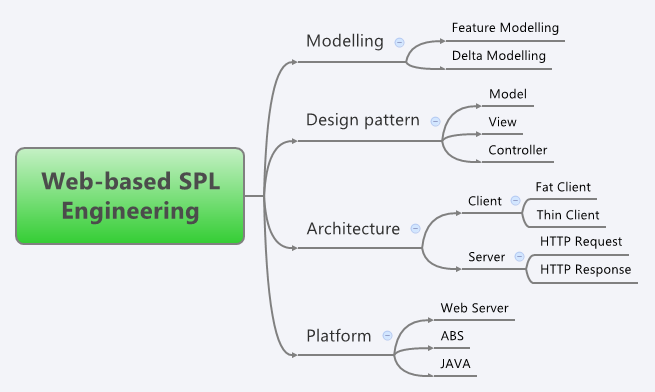
\includegraphics[width=0.8\textwidth]
        {img/kerangka-berpikir.png}
    \caption{Kerangka berpikir}
\end{figure}

\noindent
Setelah penulis mengetahui solusi apa yang harus digunakan agar ABS dapat berjalan di \textit{Application Server}, selanjutnya penulis akan merancang bagaimana pengorganisasian kode yang baik untuk ABS agar sesuai dengan kaidah MVC. Hal ini perlu dilakukan karena nantinya penelitian ini akan menghasilkan sebuah \textit{framework} MVC yang akan digunakan dalam pengembangan SPL berbasis web dengan menggunakan ABS. Dalam hal ini, penulis harus mengkaji terkait peran-peran setiap komponen pada MVC dan kemudian mengimplementasikannya ke ABS. \\

\noindent
Rangkaian proses diatas diharapkan nantinya menghasilkan sebuah framwork MVC yang utuh untuk kemudian diintegrasikan dengan konsep \textit{feature modelling} dan \textit{delta modelling} yang ada di ABS. Hal ini dilakukan agar dapat dihasilkan sebuah framework MVC ABS yang dapat digunakan untuk keperluan pengembangan SPL berbasis web.

%---------------------------------------------------------
\section{Sistematika Penulisan}
%---------------------------------------------------------
berikut adalah sistematika penulisan dari proposal ini:
\begin{itemize}
    \item Bab 1 \babSatu \\
    Bab ini berisi tentang latar belakang penelitian, manfaat penelitian, kerangka berpikir, dan sistematika penulisan.
    \item Bab 2 \babDua \\
    Bab ini berisi tentang hasil studi literatur yang dilakukan oleh penulis baik terkait teori-teori dasar yang mendukung penelitian ini ataupun peneletian lain yang masih berkaitan dengan penelitian yang akan dilakukan.
    \item Bab 3 \babTiga \\
    Bab ini berisi tentang rumusan masalah dari penelitian yang akan dilakukan, ruang lingkup penelitian, serta batasan penelitian.
    \item Bab 4 \babEmpat \\
    Bab ini berisi tentang rancangan penelitian yang akan dilakukan oleh penulis dan penjelasan dari setiap tahapan-tahapan yang akan dilakukan.
    \item Bab 5 \babLima \\
    Bab ini berisi penegasan kembali terkait rumusan masalah dan tahapan penelitian yang diambil untuk mencari solusi dari permasalahan-permasalahan tersebut.
\end{itemize}
\chapter{\babDua}

%---------------------------------------------------------
\section{Model View Controller}
%---------------------------------------------------------
\noindent
\textit{Model-View-Controller} (MVC) atau yang biasa juga dikenal dengan sebutan \textit{Presentation-Abstraction-Control} (PAC) merupakan salah satu pendekatan dalam proses pengembangan perangkat lunak yang ditujukan untuk melakukan pemisahan antara logika aplikasi, data, dan presentasi. Konsep ini dibangun atas kesadaran bahwa sebuah model domain aplikasi yang sama dapat disajikan dan diperlakukan secara berbeda tergantung dari kebutuhan si pengguna aplikasi. Dengan menggunakan pendekatan ini, seorang pengembang perangkat lunak dapat berfokus pada satu bagian saja tanpa harus mengkhawatirkan akan terkena dampak perubahan ataupun memberikan perubahan ke bagian aplikasi lainnya.

\subsection{Sejarah Singkat MVC}
\noindent
Konsep MVC diterapkan pertama kalinya oleh Alan Kay, Dan Ingalls, dan Adele Goldberg pada tahun 1980 ketika mereka merancang bahasa pemrograman smalltalk-80 di Xerox PARC Learning Research Group (LRG) \citep{krasner1988desc}. bahasa pemrograman ini didesain dan dikembangkan dengan menggunakan strategi yang merepresentasikan informasi, tampilan, dan kontrol pada lingkungan pemrogramannya. Strategi ini digunakan dengan tujuan (1) untuk membuat kumpulan komponen sistem spesial yang dibutuhkan dalam mendukung proses pengembangan perangkat lunak yang interaktif serta (2) menyediakan kumpulan komponen sistem umum yang dapat membantu pengembang dalam menciptakan aplikasi grafis yang interaktif dengan mudah \citep{krasner1988desc}. Strategi dan tujuan tersebut dibuat dalam rangka menjawab isu utama dalam pengembangan perangkat lunak yaitu terkait pemanfaatan kembali komponen yang telah dibuat (\textit{reusability}) dan kemudahan dalam menggabungkan setiap komponen aplikasi (\textit{plugability}). \\

\noindent
Belajar dari pengalamannya dalam mengembangkan smalltalk-76, para pengembang smalltalk-80 menemukan bahwa untuk mencapai sebuah modularitas yang tinggi diperlukan adanya tiga buah pemisahan fokus dalam pengembangan aplikasi. Tiga buah pemisahan fokus tersebut antara lain adalah (1) memisahkan setiap komponen yang merepresentasikan model domain aplikasi dengan (2) cara yang digunakan untuk merepresentasikan model tersebut ke pengguna aplikasi dan (3) cara yang digunakan oleh pengguna dalam berinteraksi dengan model tersebut. Tiga buah pemisahan tersebut dapat terangkum dalam sebuah konsep yang disebut dengan \textit{Model-View-Controller} (MVC).

\subsection{Penerapan MVC dalam Pengembangan Aplikasi Web}
Aplikasi web merupakan aplikasi yang tergolong interaktif karena aplikasi jenis ini banyak memiliki elemen-elemen yang dapat digunakan untuk berinteraksi dengan penggunannya. Sebagai contoh, dalam sebuah halaman situs web tentunya kita akan menemukan banyak tombol, gambar, tautan, dan kotak isian yang dapat kita gunakan untuk berinteraksi dengan situs web tersebut. Untuk sebuah aplikasi yang tergolong interaktif, adanya pemisahan antara logika aplikasi, data, dan presentasi tentunya akan dapat meningkatkan fleksibilitas aplikasi tersebut dari segi pengembangan. \\

\noindent
Pada dasarnya, arsitektur apliksi berbasis web terbagi menjadi dua bagian yaitu \textit{client} dan \textit{server}. Dengan arsitektur yang seperti ini, para pengembang aplikasi tidak dapat menentukan dengan jelas bagaimana bentuk partisi yang harus dibuat untuk aplikasi tersebut. Sebagai contoh, dengan adanya pembagian antara \textit{client} dan \textit{server}, para pengembang aplikasi harus menentukan dimanakah komponen \textit{view} akan dibentuk? Apakah komponen ini akan dibentuk di tingkat \textit{client} ataukah di tingkat \textit{server}. Begitupun dengan komponen \textit{Model} dan \textit{Controller
}-nya. Apakah komponen-komponen tersebut akan akan dibuat di tingkat \textit{client}, \textit{server}, atau keduanya? Pada akhirnya, keputusan dalam menentukan skema partisi yang dipakai akan sangat bergantung pada teknologi yang digunakan \citep{leff2001web}. \\

\noindent
Permasalahan terkait pemisahan antara \textit{client} dan \textit{server} pada aplikasi berbasis web menjadikan penerapan MVC lebih sulit. Proses penerapan MVC akan dapat berhasil apabila (1) para pengembang aplikasi sudah mengetahui bagaimana skema partisi yang akan diterapkan serta (2) teknologi dan infrastruktur yang ada \textit{compatible} dengan skema partisi yang diterapkan. Oleh karena itu, perlu adanya sebuah pendekatan yang dapat digunakan oleh para pengembang untuk memastikan dua hal tersebut.

%---------------------------------------------------------
\section{Software Product Line Engineering (SPLE)}
%---------------------------------------------------------
\noindent
\textit{Software Product Line Engineering} (SPLE) merupakan sebuah paradigma yang digunakan dalam proses pengembangan perangkat lunak dengan menggunakan prinsip \textit{platform} dan \textit{mass customisation} \citep[p.~14]{pohl2005software}. Dalam industri perangkat lunak, istilah \textit{platform} atau \textit{software platform} biasa diartikan sebagai sebuah sistem komputer (misal: prosesor atau kombinasi antara perangkat keras dengan sistem operasi) yang menyebabkan dapat berjalannya sebuah program komputer. Sedangkan dalam konteks SPLE, yang dimaksud dengan \textit{platform} adalah sebuah subsistem dan \textit{interface} yang membentuk sebuah struktur umum dimana nantinya sebuah produk turunan dapat dikembangkan dan diproduksi secara efisien \citep[p.~15]{pohl2005software}. \\

\noindent
Dalam paradigma SPLE, proses pengembangan perangkat lunak dibagi menjadi dua bagian yaitu \textit{Domain Engineering} dan \textit{Application Engineering} \citep[p.~21]{pohl2005software}. \textit{Domain Engineering} adalah sebuah proses dalam SPLE dimana pada tahap ini seluruh \textit{commonality} dan \textit{variability} dari SPL didefinisikan dan direalisikan. Sedangkan tahap \textit{Application Engineering} adalah sebuah proses dimana aplikasi dari SPL dibuat dengan cara memanfaatkan \textit{domain artifact} yang telah dibuat pada tahap sebelumnya dan mengeksploitasi \textit{variability} yang ada di dalam SPL tersebut. Tahapan-tahapan proses dalam SPLE ini biasa disebut dengan istilah \textit{SPLE Framework}. \\

\begin{figure}
    \centering
    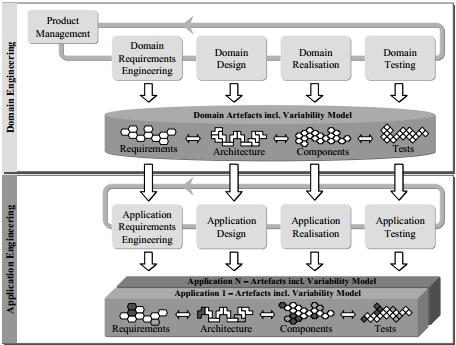
\includegraphics[width=0.8\textwidth]
        {img/sple-process.png}
    \caption{SPLE Framework}
\end{figure}
\vspace{-0.8cm}
\begin{center}
{\small Sumber gambar: \citep{pohl2005software}}
\end{center}

%---------------------------------------------------------
\section{Abstract Behavioural Spesification (ABS)}
%---------------------------------------------------------
\noindent
Abstract Behavioural Specification Language (ABS) merupakan sebuah bahasa pemodelan yang dibuat oleh konsorsium uni eropa di bawah proyek bernama \textit{Highly Adaptable and Trustworthy Software using Formal Method} (HATS). Tujuan dari proyek HATS dalam menciptakan ABS adalah untuk menciptakan sebuah pendekatan yang \textit{model-centric} dalam melakukan proses perancangan, implementasi dan verifikasi dari sebuah sistem yang \textit{highly-configurable} \citep{clarke2012variability}. Pada dasarnya ABS dibagi kedalam beberapa layer (lihat gambar 2.x) yang diantaranya adalah \textit{functional abstraction}, \textit{OO-Imperative layer}, \textit{Concurency Model} dan \textit{ABS Core}. \\

\begin{figure}
    \centering
    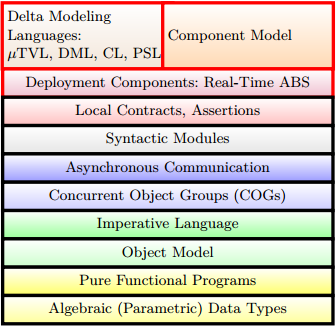
\includegraphics[width=0.6\textwidth]
        {img/abs-layers.png}
    \caption{ABS Layer}
\end{figure}
\vspace{-0.8cm}
\begin{center}
{\small Sumber gambar: \citep{hahnle2013hats}}
\end{center}

\noindent
Sebagai sebuah bahasa pemrograman \textit{imperative} yang menganut konsep \textit{Object Oriented}, secara umum ABS memiliki sintaks yang sama dengan bahasa pemrograman JAVA (walaupun lebih sederhana). Salah satu perbedaan yang paling mendasar antara ABS dengan JAVA adalah pada konsep \textit{code reuse}-nya. Pada bahasa pemrograman JAVA, konsep \textit{code reuse} diimplementasikan dengan cara membuat \textit{code inheritance} sedangkan pada ABS konsep tersebut diimplementasikan dalam betuk \textit{code deltas} \citep{hahnle2013hats}. \textit{code deltas} pada ABS merupakan sebuah kumpulan kode yang mendeskripsikan perubahan-perubahan kode pada kelas yang dituju. Dengan adanya konsep ini, ABS dapat melakukan manipulasi kelas seperti menambah atau menghilangkan \textit{variable} dan \textit{method}. \\

\noindent
Seperti yang sudah disebutkan sebelumnya bahwa di dalam ABS konsep \textit{code reuse} diimplementasikan dalam bentuk \textit{code deltas}. \textit{Code deltas} tersebut nantinya akan digunakan untuk memodelkan \textit{variability} yang terjadi di tingkat \textit{source code}. pemodelan \textit{variability} ini merupakan sebuah pendekatan yang dilakukan oleh ABS dalam membangun sebuah SPL. Proses pemodelan \textit{variability} ini biasa disebut juga sebagai proses \textit{Delta Modelling}. \\

\noindent
\textit{Delta Modelling} merupakan sebuah pendekatan yang fleksible dan modular dalam mewujudkan berbagai macam variasi produk dengan menggunakan kembali artifak-artifak yang ada \citep{hahnle2013hats}. Dalam proses \textit{Delta Modelling}, realisasi dari SPL dibentuk dari dua bagian yaitu \textit{core module} dan \textit{delta module}. \textit{Delta module} berisi fungsi-fungsi yang berlaku umum terhadap semua varian produk yang akan dibuat sedangkan \textit{delta modul} merupakan enkapsulasi dari perubahan-perubahan yang akan terjadi pada \textit{core product} untuk kemudian menghasilkan varian produk yang lain. \\

\begin{figure}
    \centering
    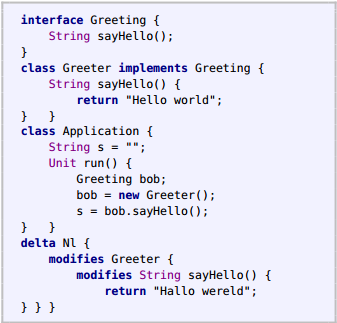
\includegraphics[width=0.6\textwidth]
        {img/delta-modelling-1.png}
\end{figure}

\begin{figure}
    \centering
    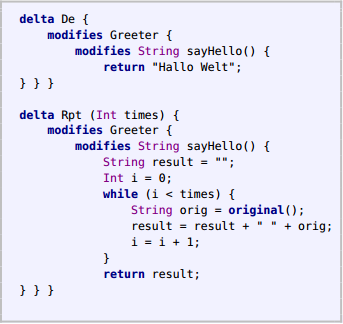
\includegraphics[width=0.6\textwidth]
        {img/delta-modelling-2.png}
    \caption{Delta Modelling pada ABS}
\end{figure}\vspace{-0.8cm}
\begin{center}
{\small Sumber gambar: \citep{clarke2012variability}}
\end{center}
\chapter{\babTiga}

%---------------------------------------------------------
\section{Eksperimen Awalan}
%---------------------------------------------------------
Sebelum penulis membuat proposal, penulis telah melakukan beberapa eksperimen kecil untuk mengetahui seberapa memungkinkannya ABS digunakan untuk pengembangan aplikasi berbasis web. Penelitian kecil yang telah dilakukan antara lain adalah:

\begin{enumerate}
    \item Mencoba fitur-fitur ABS seperti \textit{feature modelling} dan \textit{delta modelling} dengan menggunakan studi kasus sederhana. Tujuan dilakukannya eksperimen ini adalah untuk melakukan eksplorasi terkait fitur \textit{delta modelling} dan \textit{feature modelling} ABS yang nantinya akan digunakan untuk membuat SPL.
    \item Mencoba menggabungkan kelas JAVA yang dihasilkan ABS dengan framework web berbasis JAVA seperti JAVA Servlet dan Play Framework. Tujuan dilakukannya ekperimen ini adalah untuk melihat apakah file JAVA yang dihasilkan oleh ABS dapat langsung dimasukkan ke dalam \textit{framework} dan web server yang sudah seperti Tomcat atau Play Framework. Setelah dilakukan beberapa kali percobaan pada akhirnya penulis berkesimpulan bahwa framework dan web server tersebut tidak \textit{compatible} dengan file JAVA yang dihasilkan oleh ABS.
    \item Mencoba membuat web server sendiri yang dapat digunakan untuk memproses \textit{HTTP Request} dan kemudian memanggil ABS untuk membuat \textit{HTTP Response}-nya. Tujuan dari dilakukannya eksperimen ini adalah untuk mencari solusi alternatif setelah eksperimen yang sebelumnya belum berhasil menghasilkan sebuah solusi. Dalam eksperimen ini penulis membuat sebuah web server sederhana dengan menggunakan bahasa pemrograman JAVA yang kemudian dijalankan dengan menggunakan runtime ABS. Sampai sejauh ini, pendekatan yang penulis lakukan sudah membuahkan hasil yaitu penulis dapat menghasilkan sebuah \textit{HTTP response} berupa halaman HTML yang dibuat oleh ABS.
    \item Mencoba untuk mengorganisasikan kelas-kelas yang dibuat dengan menggunakan ABS agar sesuai dengan kaidah MVC. Eksperimen ini dilakukan untuk mendapatkan gambaran awal bagaimana cara menghubungkan kelas \textit{Model-View-Controller}  yang telah dibuat.
\end{enumerate}

\begin{figure}
    \centering
    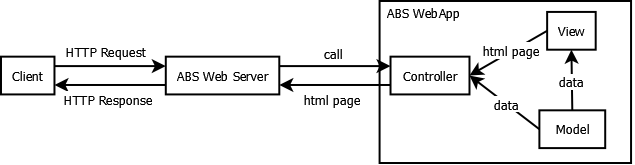
\includegraphics[width=0.8\textwidth]
        {img/abs-mvc.png}
    \caption{Skema framework ABS}
\end{figure}

\begin{figure}
    \centering
    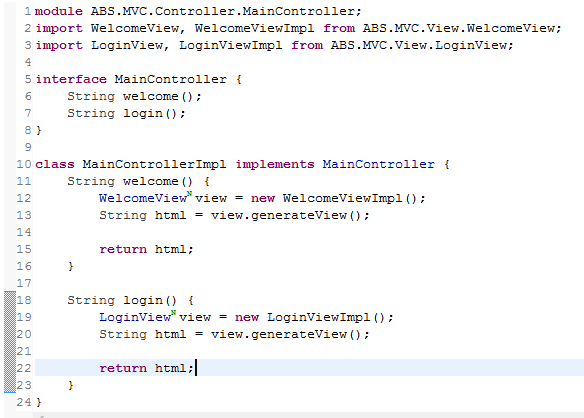
\includegraphics[width=0.8\textwidth]
        {img/controller-eksperimen.png}
    \caption{Contoh Controller}
\end{figure}

\begin{figure}
    \centering
    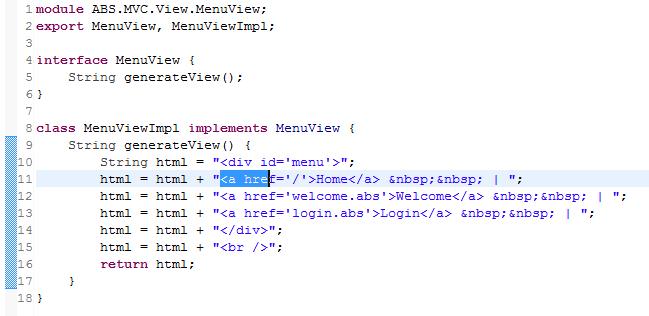
\includegraphics[width=0.8\textwidth]
        {img/view-eksperimen.png}
    \caption{Contoh ABS View}
\end{figure}

\begin{figure}
    \centering
    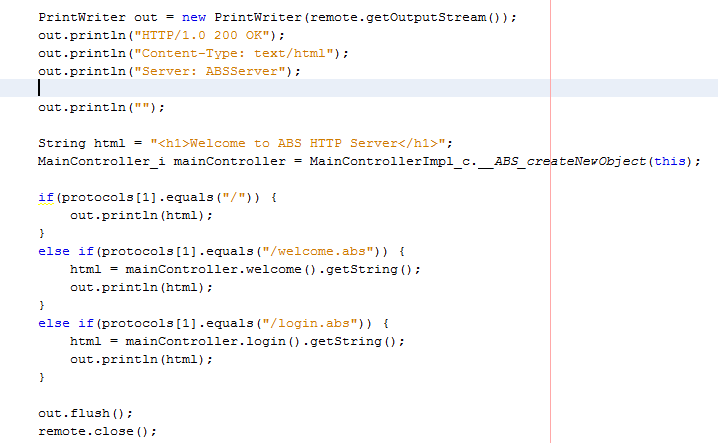
\includegraphics[width=0.8\textwidth]
        {img/server-eksperimen.png}
    \caption{Contoh ABS Server yang dibuat}
\end{figure}

\begin{figure}
    \centering
    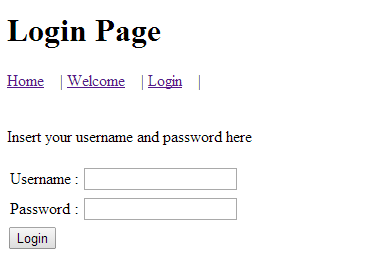
\includegraphics[width=0.8\textwidth]
        {img/login-page.png}
    \caption{Contoh halaman HTML yang dihasilkan dari ABS}
\end{figure}

%---------------------------------------------------------
\section{Rumusan Masalah}
%---------------------------------------------------------
\noindent
Berikut ini adalah rumusan masalah yang diperoleh dari hasil studi literatur dan percobaan awalan yang telah dilakukan oleh penulis sampai saat ini:

\begin{enumerate}
    \item Bagaimana strategi yang tepat dalam melakukan pemetaan bahasa pemodelan ABS ke dalam pola Model, View dan Controller dengan tetap mempertahankan kaidah-kaidah yang ada sesuai dengan studi literatur yang telah dilakukan.
    \item Arsitektur perangkat lunak seperti apakah yang cocok untuk pengembangan SPL berbasis dengan menggunakan bahasa pemodelan ABS.
    \item Bagaimana strategi implementasi yang dapat dilakukan agar \textit{framework} ABS yang dibuat dapat mendukung fitur \textit{delta modelling} yang dimiliki oleh ABS. 
\end{enumerate}

%---------------------------------------------------------
\section{Ruang Lingkup Penelitian}
%---------------------------------------------------------
\noindent
Adapun ruang lingkup dari penelitian ini adalah tentang perancangan dan perumusan strategi pengembangan \textit{framework} MVC SPL berbasis web dengan menggunakan bahasa pemodelan ABS. Harapannya, melalui penelitian ini penulis dapat menghasilkan sebuah \textit{framework} ABS yang dapat digunakan untuk melakukan pengembangan SPL berbasis web dengan menggunakan bahasa pemodelan ABS. Berdasarkan ruang lingkup tersebut, maka poin-poin pengerjaan yang akan dilakukan oleh penulis dalam penelitian ini antara lain adalah:

\begin{enumerate}
    \item Melakukan analisa terhadap sintaks dan aturan-aturan yang berlaku pada bahasa pemodelan ABS untuk kemudian dapat dirumuskan strategi dalam melakukan pemetaan bahasa pemodelan ABS kedalam komponen-komponen \textit{Model, View} dan \textit{Controller}.
    \item Merancang arsitektur dan strategi pengembangan \textit{framewok} ABS agar dapat mendukung fitur \textit{delta modelling} yang dimiliki oleh ABS.
    \item Membuat framework ABS berdasarkan strategi dan rancangan yang telah dilakukan sebelumnya.
\end{enumerate}

%---------------------------------------------------------
\section{Batasan Penelitian}
%---------------------------------------------------------

Dikarenakan adanya keterbatasan dalam hal pengetahuan, waktu pengerjaan dan fokus pengerjaan maka penulis menentukan batasan-batasan penelitian untuk penelitian kali ini yang diantaranya adalah:

\begin{enumerate}
    \item \textit{Framework} yang dibuat belum mendukung akses database karena untuk masalah akses \textit{database} pada ABS sudah menjadi topik penelitian tersendiri.
    \item \textit{Web Server} yang dibuat hanya berupa \textit{web server} sederhana dengan fungsionalitas terbatas pada menerima \textit{HTTP Request}, meneruskan \textit{request} tersebut ke ABS, serta mengirimkan \textit{HTTP Response} yang diberikan oleh ABS ke web browser. Oleh karena itu, penulis tidak akan mempertimbangkan masalah keamanan data, efisiensi dari \textit{web server} ataupun masalah \textit{concurency access} pada \textit{web server}.
    \item Penulis tidak melakukan komparasi antara \textit{framework} MVC yang dibuat dengan \textit{framework} MVC sejenis dikarenakan masih minimnya literatur yang membahas tentang pengembangan \textit{framework} MVC SPL berbasis web untuk bahasa pemodelan ABS.
\end{enumerate}

%---------------------------------------------------------
\section{Potensi Hambatan}
%---------------------------------------------------------

Adapun potensi hambatan yang diperkirakan akan muncul selama menjalani proses penelitian ini antara lain adalah:

\begin{enumerate}
    \item Sulitnya mendapatkan narasumber yang dapat ditanyakan tentang detail dari bahasa pemodelan ABS itu sendiri. Hal ini terjadi dikarenakan para ahli yang mengerti secara detail tentang bahasa pemodelan ABS semuanya berada di Eropa.
    \item Minimnya literatur tentang pemanfaatan bahasa pemodelan ABS untuk pengembangan SPL berbasis web.
\end{enumerate}
\chapter{\babEmpat}

Berdasarkan rumusan masalah, ruang lingkup penelitian, serta batasan penelitian yang sudah dibahas pada bab sebelumnya, berikut ini adalah rancangan penelitian yang akan dilakukan:

\begin{figure}
    \centering
    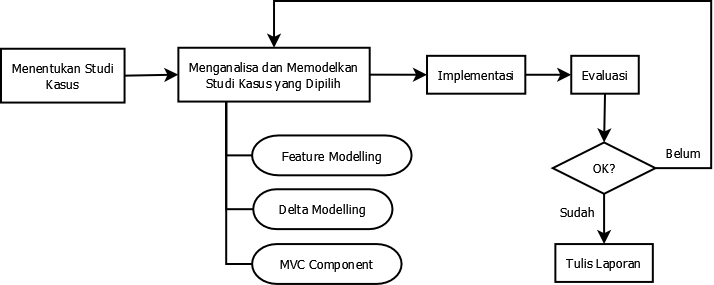
\includegraphics[width=0.8\textwidth]
        {img/alur-penelitian.png}
    \caption{Rencana Penelitian}
\end{figure}

\noindent
Di awal penelitian, penulis akan melakukan fiksasi studi kasus yang akan digunakan dalam penelitian ini. Setelah proses fiksasi studi kasus, berikutnya penulis akan melakukan analisis studi kasus tersebut serta memodelkan solusi yang akan dibuat. Hasil dari proses analisi ini adalah berupa diagram \textit{feature modelling}, \textit{delta modelling} dan daftar komponen-komponen MVC yang akan dibuat. Langkah selanjutnya adalah mengimplementasikan model yang sudah dibuat agar nantinya dapat diperoleh sebuah \textit{framework} ABS MVC yang utuh sesuai dengan hasil analisa dan pemodelan dari studi kasus pada tahap sebelumnya. langkah terakhir adalah melakukan uji kelayakan dari \textit{framework} yang selesai dibuat. Apabila \textit{framework} yang dihasilkan belum memenuhi syarat kelayakan, maka penulis akan melakukan proses analisa dan pemodelan kembali untuk dapat memperbaiki framework yang ada.

%---------------------------------------------------------
\section{Fiksasi Studi Kasus}
%---------------------------------------------------------
Pada tahap ini penulis akan menentukan studi kasus seperti apa yang akan digunakan dalam penelitian ini. Studi kasus yang digunakan pada tahap ini bukanlah sebuah studi kasus yang komperhensif melainkan hanya digunakan untuk mensimulasikan strategi pengembangan SPL berbasis web dengan menggunakan framework yang telah dibuat. Dalam penelitian ini penulis akan membuat sebuah aplikasi keuangan berbasis web yang ditujukan untuk mengelola dana donasi sebuah lembaga kemanusiaan. Adapun fitur-fitur yang akan dibuat dalam studi kasus kali ini antara lain adalah:

\begin{enumerate}
    \item \textit{Create, Retrieve, Update} dan \textit{Delete} (CRUD) data dotanur lembaga.
    \item CRUD data program sosial lembaga.
    \item Laporan pengeluaran dana donasi.
    \item Laporan pemasukan dana donasi.
\end{enumerate} 

%---------------------------------------------------------
\section{Melakukan Analisa dan Pemodelan}
%---------------------------------------------------------
Pada tahap ini penulis akan mencoba menganalisa studi kasus yang dipilih terkait dengan fitur-fitur apa saja yang harus dibuat, variasi fungsi seperti apakah yang dapat dibuat dari studi kasus tersebut, serta skema partisi yang akan digunakan dalam tahap pengembangannya. Setelah selesai melakukan analisa, berikutnya adalah memodelkan studi kasus tersebut berdasarkan hasil analisa yang diperoleh sehingga nantinya akan dihasilkan sebuah \textit{feature model}, \textit{delta model}, dan daftar komponen MVC yang harus dibuat untuk studi kasus tersebut.

%---------------------------------------------------------
\section{Implementasi}
%---------------------------------------------------------
Pada tahap ini penulis mulai mengimplementasikan model-model yang sudah dibuat pada tahap sebelumnya. Proses implementasi yang dimaksud adalah mulai membuat kode-kode ABS yang dibutuhkan sesuai dengan model yang telah dibuat serta membuat \textit{web server} sederhana yang nantinya akan digunakan untuk menguji coba SPL berbasis web yang dihasilkan.

%---------------------------------------------------------
\section{Evaluasi}
%---------------------------------------------------------
Pada tahap ini penulis akan melakukan evaluasi terhadap SPL berbasis web yang telah berhasil dibuat pada tahap implementasi. Salah satu faktor yang dinilai pada tahap evaluasi ini adalah terkait kesesuaian aplikasi dengan model atau rancangan yang sudah ditentukan pada tahap analisa dan pemodelan. Apabila hasil evaluasi dari aplikasi yang dibuat belum memuaskan, maka harus ada proses analisa dan pemodelan kembali untuk melihat apakah ada bagian yang harus direvisi atau tidak. Jika hasil evaluasi aplikasi sudah memuaskan maka selanjutnya adalah menuliskan laporan penelitian. \\

\noindent
Berikut ini adalaha syarat kelayakan yang akan dijadikan parameter dalam tahap evaluasi ini:

\begin{enumerate}
    \item Apakah \textit{framework} yang dihasilkan sudah sesuai dengan kaidah MVC yang berlaku? (sesuai dengan yang ada pada studi literatur)
    \item Apakah \textit{framework} yan dihasilkan dapat diintegrasikan dengan \textit{feature modelling} dan \textit{delta modelling} pada ABS?
    \item Apakah \textit{framework} yang dihasilkan sudah dapat mengasilkan sebuah \textit{complete product} SPL berbasis web? (dapat dijalankan)
\end{enumerate}

%---------------------------------------------------------
\section{Penulisan Laporan}
%---------------------------------------------------------
Pada tahap ini penulis akan menuliskan laporan penelitian dan menarik kesimpulan yang diambil dari penelitian yang sudah dilakukan serta memaparkan temuan-temuan yang diperoleh selama melakukan penelitian.
\chapter{\babLima}

Penelitian ini bertujuan untuk membuat sebuah \textit{framework} MVC yang akan digunakan dalam proses pengembangan SPL berbasis web dengan ABS. Berdasarkan pemaparan pada bab-bab sebelumnya, tujuan dari penelitian ini mencakup beberapa hal yang diantaranya adalah:

\begin{enumerate}
    \item Membuat \textit{web server} sederhana yang dapat digunakan untuk menjalankan SPL berbasis web yang dibuat dengan menggunakan ABS.
    \item Membuat \textit{framework} MVC untuk ABS yang berisi abstraksi untuk menghasilkan halaman ABS, mengakses data, serta \textit{URL routing} yang dapat digunakan oleh para pengembang untuk mengembangkan SPL berbasis web dengan menggunakan ABS.
    \item Membuat \textit{tools} yang dapat digunakan untuk melakukan proses integrasi dan \textit{deployment}.
\end{enumerate}

\noindent
Untuk menyelesaikan permasalahan-permasalahan di atas, maka penulis akan melakukan sebuah penelitian dengan tahapan-tahapan sebagai berikut:

\begin{enumerate}
    \item Melakukan fiksasi studi kasus.
    \item Menganalisan dan memodelkan permasalahan yang ada pada studi kasus tersebut.
    \item Mengimplementasikan hasil analisa dan pemodelan dari studi kasus untuk menghasilkan sebuah \textit{framework} MVC yang utuh.
    \item Mengevaluasi \textit{framework} yang telah berhasil dibuat.
    \item Menuliskan laporan hasil penelitian yang telah dilakukan.
\end{enumerate}

\bibliography{conf/bib}
\bibliographystyle{conf/apalikerd}

\end{document}